\titre{}
\theme{derivation}
\auteur{Nathan Scheinmann}
\niveau{2M}
\source{crm}
\type{serie}
\piments{1}
\pts{}
\annee{2526}

\contenu{
\tcblower
Pour $f(x)=|2x-4|$ et $g(x)=x+1$, puis pour $f(x)=|x^2-4x|$ et $g(x)=x+2$. 
\begin{tasks}
	\task Représenter $f(x)$ et $g(x)$. 
	\task Résoudre $f(x)=g(x)$.
	\task Déterminer à l'aide des calculs et du graphique les solutions de $f(x)<g(x)$. 
\end{tasks}
}
\correction{
\tcblower
  \begin{center}
  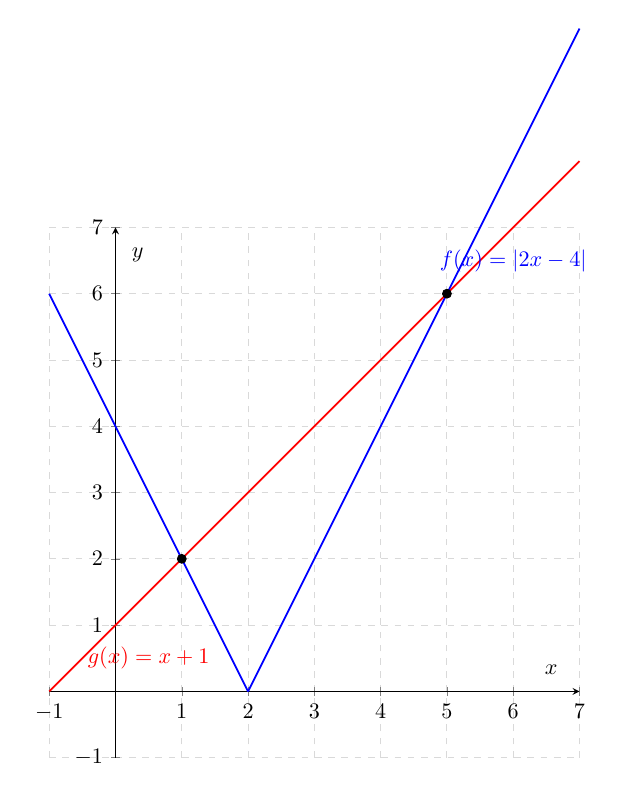
\begin{tikzpicture}[>=stealth,scale=0.8]
  \begin{axis}[
      width=10cm,height=10cm,
      axis lines=middle, axis line style={->},
      xlabel={$x$}, ylabel={$y$},
      every axis x label/.style={at={(ticklabel* cs:0.92)}, anchor=west, yshift=10pt},
      every axis y label/.style={at={(ticklabel* cs:0.92)}, anchor=south, xshift=10pt},
      xmin=-1,xmax=7, ymin=-1,ymax=7,
      xtick={-1,0,1,2,3,4,5,6,7},
      ytick={-1,0,1,2,3,4,5,6,7},
      grid=both,
      grid style={dashed,gray!30},
      clip=false]

  % Absolute value function: |2x - 4|
  \addplot[smooth,thick,domain=-1:2,samples=80,blue] {-2*x+4};
  \addplot[smooth,thick,domain=2:7,samples=80,blue] {2*x-4};

  % Linear function: g(x) = x + 1
  \addplot[smooth,thick,domain=-1:7,samples=80,red] {x+1};

  % Mark intersection points (solutions)
  \draw[fill=black] (axis cs:1,2) circle (2pt);
  \draw[fill=black] (axis cs:5,6) circle (2pt);

  % Function labels
  \node[blue] at (axis cs:6,6.5) {$f(x)=|2x-4|$};
  \node[red] at (axis cs:0.5,0.5) {$g(x)=x+1$};

  \end{axis}
  \end{tikzpicture}
  \end{center}

  Solutions: $x = 1$ and $x = 5$ (both valid)

  ---
  Equation 2: |x² - 4x| = x + 2

  \begin{center}
  \begin{tikzpicture}[>=stealth,scale=0.8]
  \begin{axis}[
      width=10cm,height=12.5cm,
      axis lines=middle, axis line style={->},
      xlabel={$x$}, ylabel={$y$},
      every axis x label/.style={at={(ticklabel* cs:0.92)}, anchor=west, yshift=10pt},
      every axis y label/.style={at={(ticklabel* cs:0.92)}, anchor=south, xshift=10pt},
      xmin=-1,xmax=7, ymin=-1,ymax=9,
      xtick={-1,0,1,2,3,4,5,6,7},
      ytick={-1,0,1,2,3,4,5,6,7,8,9},
      grid=both,
      grid style={dashed,gray!30},
      clip=false]

  % Absolute value of parabola: |x² - 4x|
  \addplot[smooth,thick,domain=-1:0,samples=80,blue] {x^2-4*x};
  \addplot[smooth,thick,domain=0:4,samples=80,blue] {-x^2+4*x};
  \addplot[smooth,thick,domain=4:7,samples=80,blue] {x^2-4*x};

  % Linear function: g(x) = x + 2
  \addplot[smooth,thick,domain=-1:7,samples=80,red] {x+2};

  % Mark intersection points (solutions)
  \draw[fill=black] (axis cs:1,3) circle (2pt);
  \draw[fill=black] (axis cs:2,4) circle (2pt);
  \draw[fill=black] (axis cs:5.372,7.372) circle (2pt);

  % Function labels
  \node[blue] at (axis cs:2.5,5.5) {$f(x)=|x^2-4x|$};
  \node[red] at (axis cs:6,1) {$g(x)=x+2$};

  \end{axis}
  \end{tikzpicture}
  \end{center}
}

